\documentclass[aspectratio=169]{beamer}

\usepackage{graphicx}
\usepackage{subfig}
\usepackage{amsmath}
\usepackage{xcolor}

\usetheme{CambridgeUS}
\usecolortheme{dolphin}
% \usecolortheme{beaver}
\AtBeginSection[ ]
{
    \begin{frame}{Outline}
        \tableofcontents[currentsection]
    \end{frame}
}
\title{Denoising Diffusion Probabilistic Models}
\author{
    Jonathan Ho\and 
    Ajay Jain\and 
    Pieter Abbeel
    }

\institute{UC Berkeley}

% \date{\today}
\date{November, 14, 2022}

\begin{document}



% Title
\begin{frame}
    \titlepage
    \begin{figure}[htbp]
        \subfloat{
            \begin{minipage}[t]{0.1\linewidth}
                \centering
                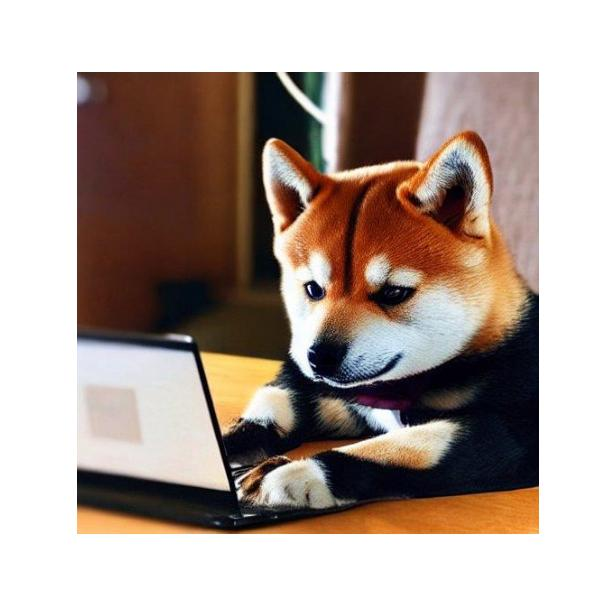
\includegraphics[width=0.7in]{../pic/dog-pictures/fig0.jpeg}
                JinYu
            \end{minipage}
        }
        \quad
        \subfloat{
            \begin{minipage}[t]{0.1\linewidth}
                \centering
                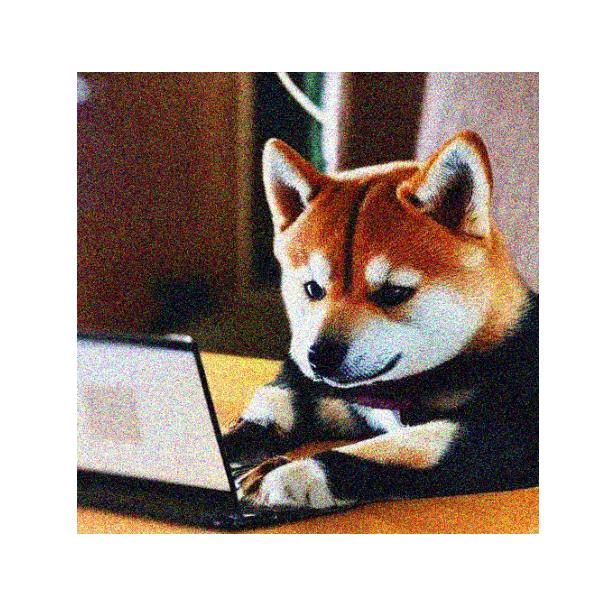
\includegraphics[width=0.7in]{../pic/dog-pictures/fig4.jpeg}
                XinkeWang
            \end{minipage}
        }
        \quad
        \subfloat{
            \begin{minipage}[t]{0.1\linewidth}
                \centering
                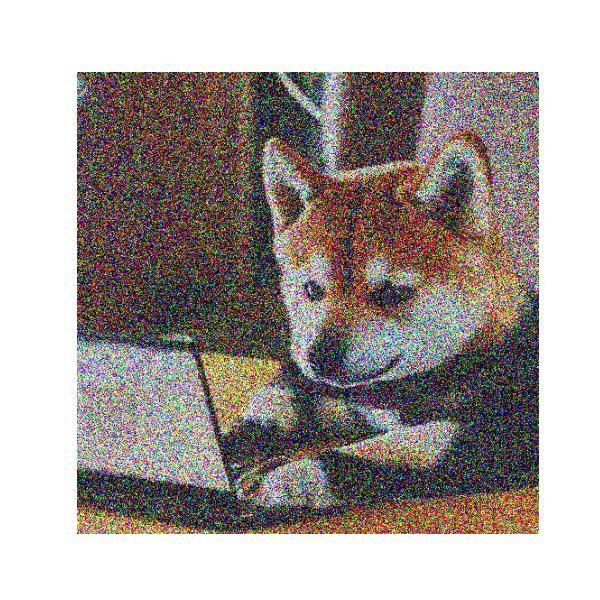
\includegraphics[width=0.7in]{../pic/dog-pictures/fig10.jpeg}
                ChangfengDuan
            \end{minipage}
        }
        \quad
        \subfloat{
            \begin{minipage}[t]{0.1\linewidth}
                \centering
                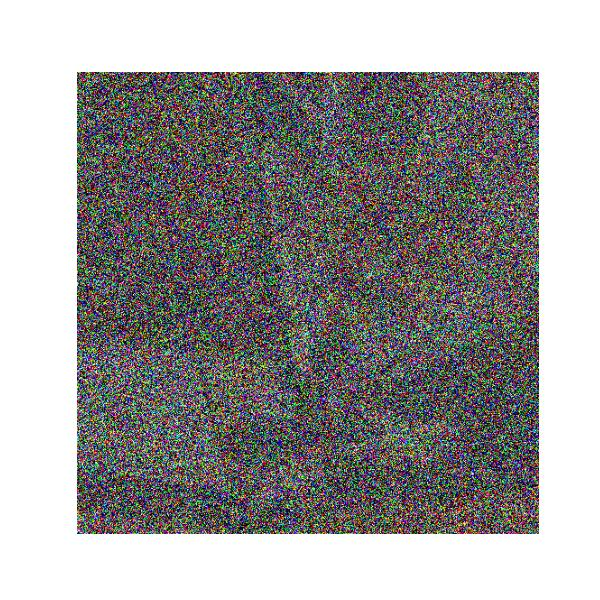
\includegraphics[width=0.7in]{../pic/dog-pictures/fig14.jpeg}
                JieLi
            \end{minipage}
        }
        \quad
        \subfloat{
            \begin{minipage}[t]{0.1\linewidth}
                \centering
                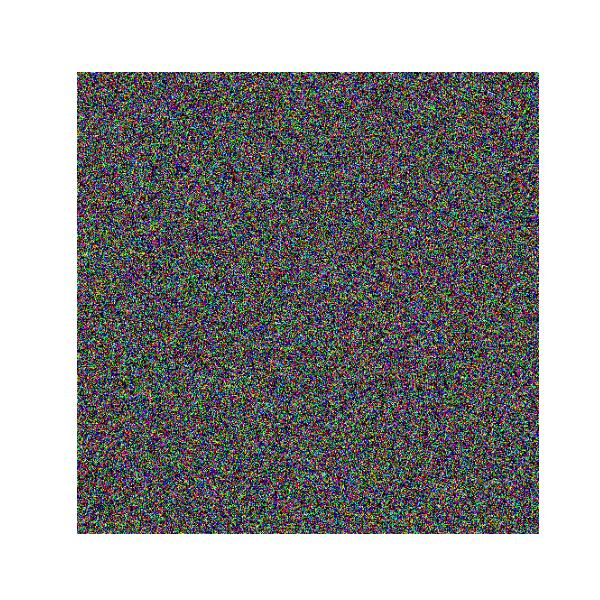
\includegraphics[width=0.7in]{../pic/dog-pictures/fig19.jpeg}
                YuhongSun
            \end{minipage}
        }
    \end{figure}
\end{frame}

\begin{frame}{Content}
    \tableofcontents[hideallsubsections]
\end{frame}

\section{Background}

\begin{frame}{What is generative model?}
    \begin{columns}
        \column{0.4\textwidth}
        \par
        Regardless of precise definition, \\ the terminology is constitutional because a generative model can be used to "generate" random instances.
        \column{0.2\textwidth}
        \begin{figure}
            \centering
            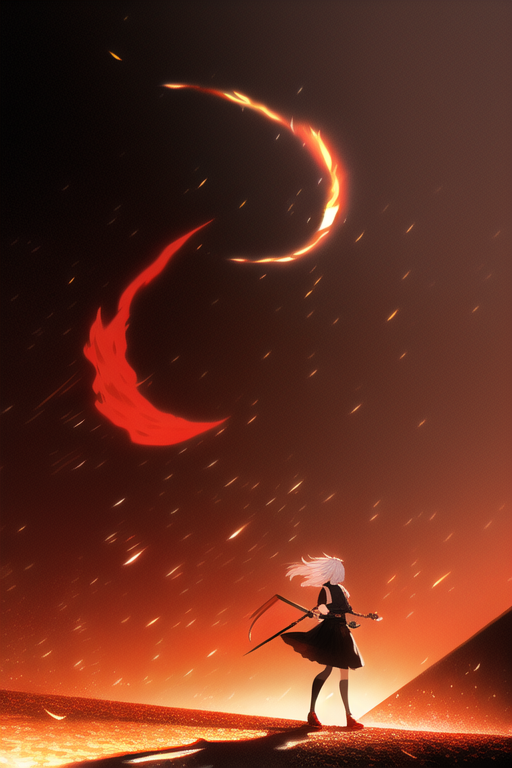
\includegraphics[width=3.3cm]{../pic/ai1.png}
            \caption{by Novel AI}
        \end{figure}
    \end{columns}
\end{frame}

\begin{frame}{Intuitive understanding}
    \begin{columns}
        \column{0.3\textwidth}
        \begin{figure}
            \centering
            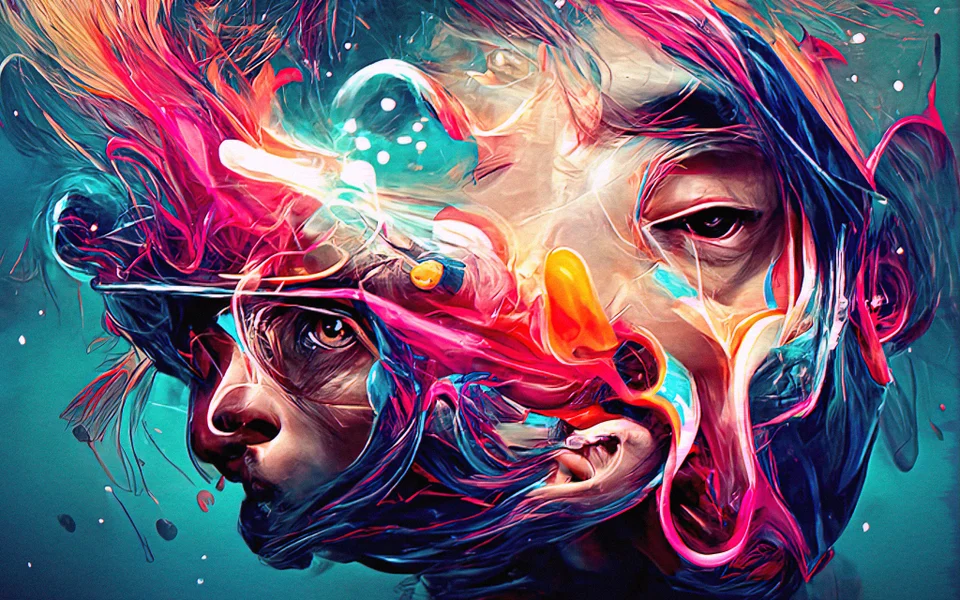
\includegraphics[width=5.5cm]{../pic/ai2.png}
            \caption{by AI}
        \end{figure}
        \column{0.3\textwidth}
        \begin{figure}
            \centering
            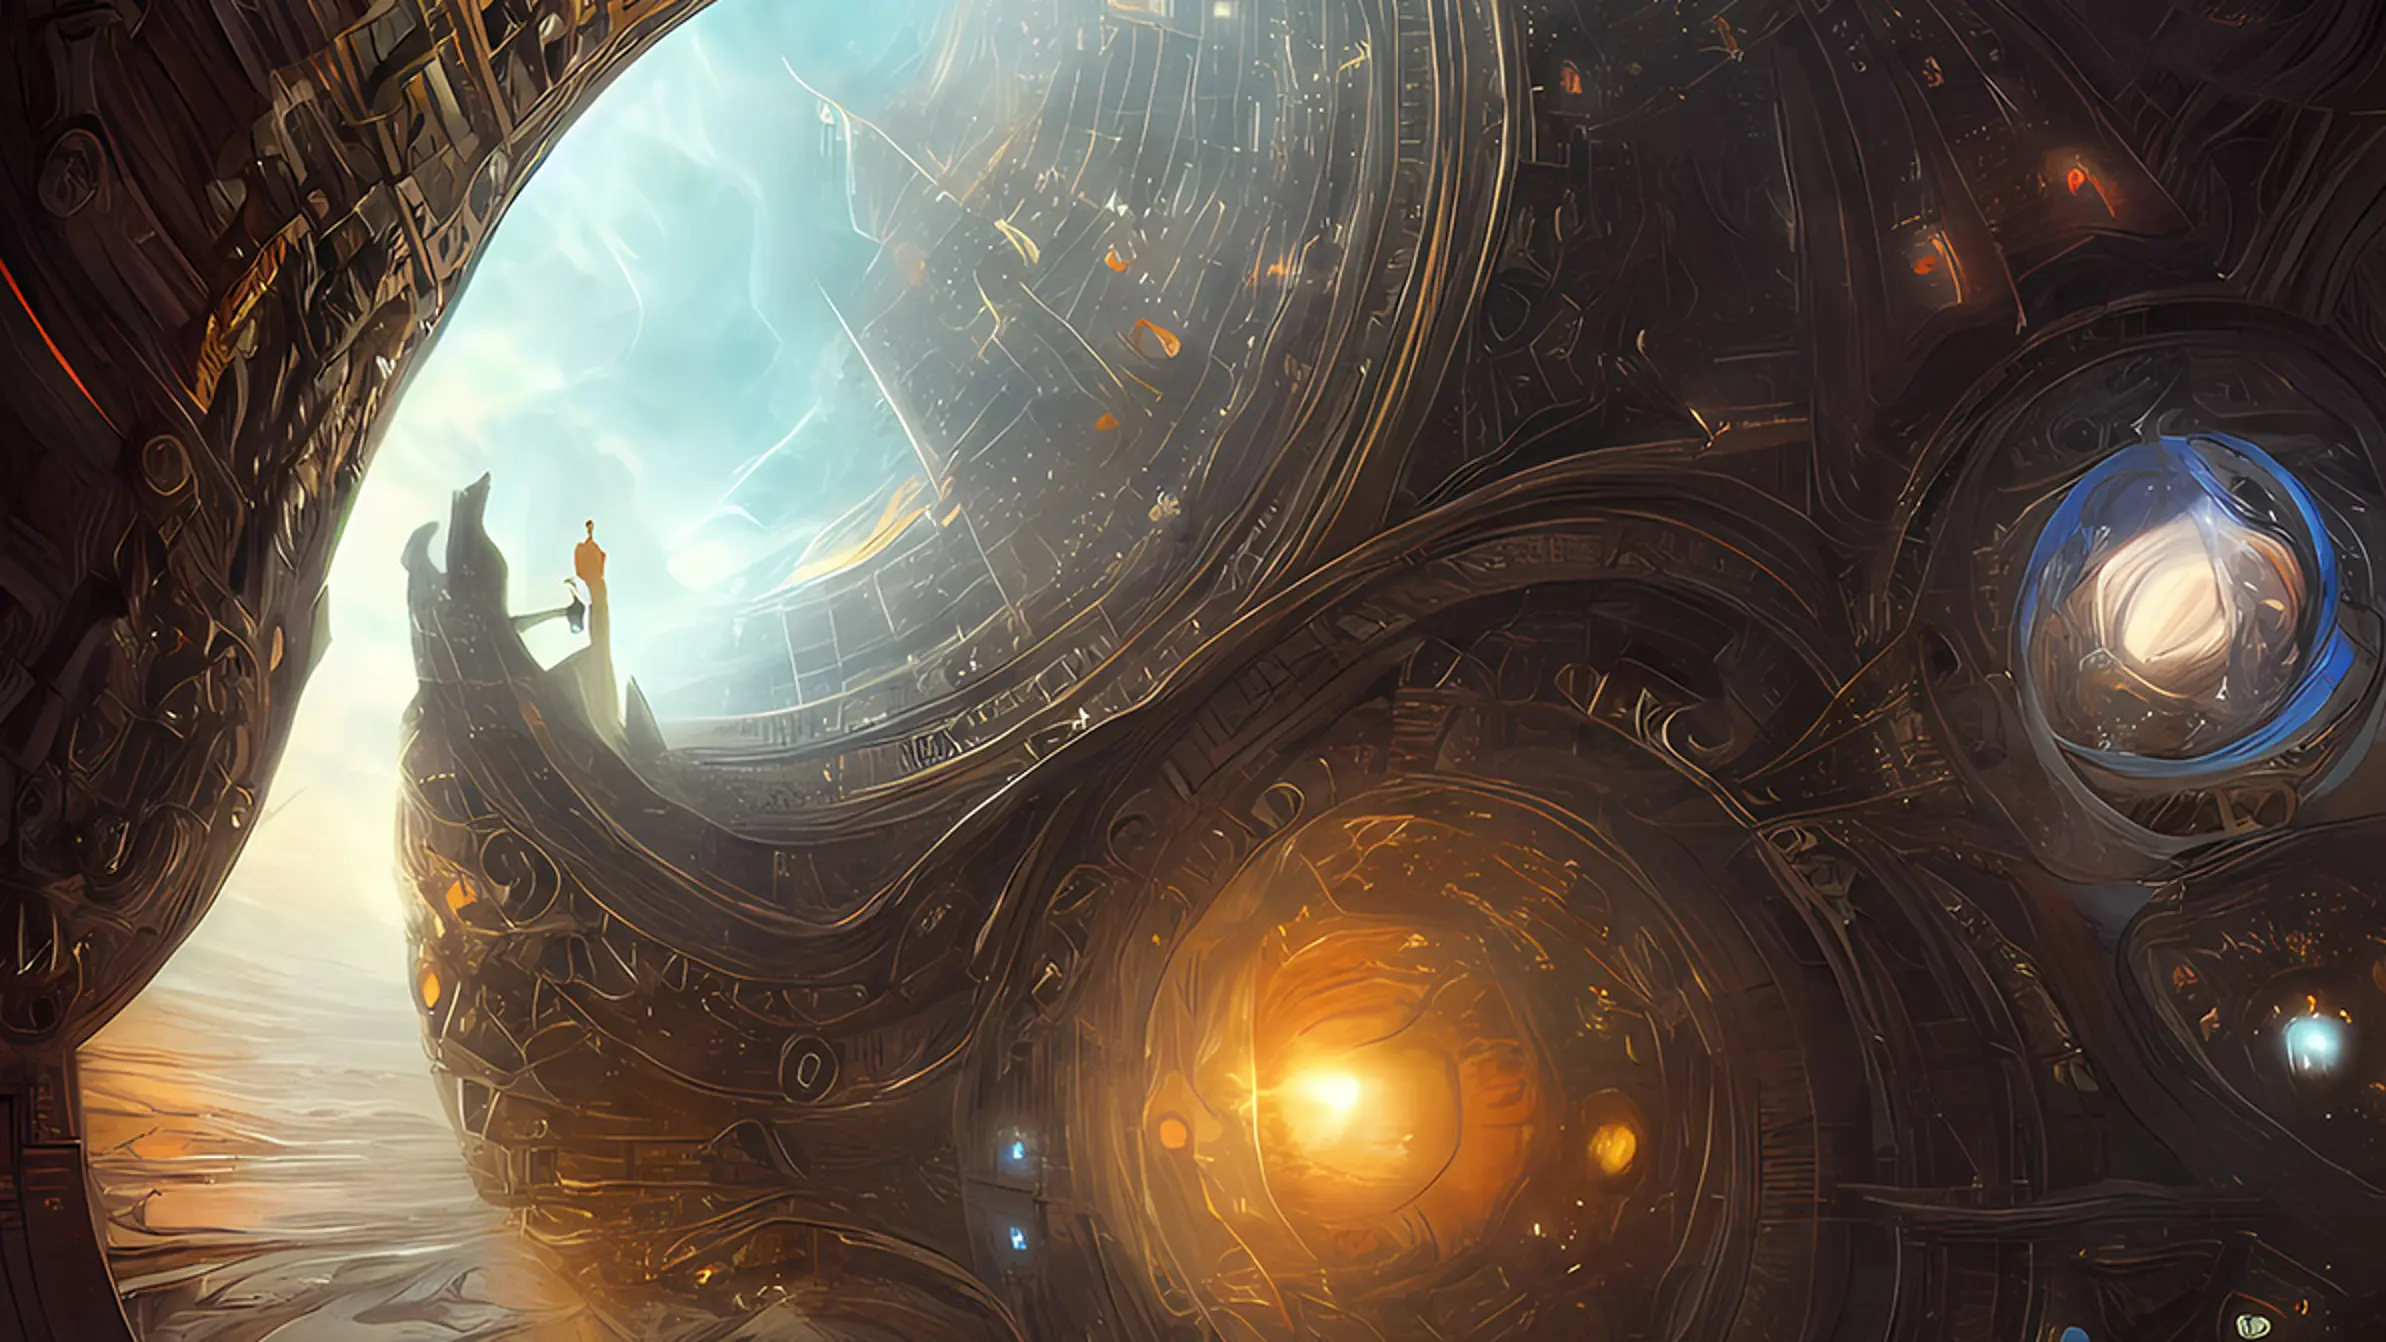
\includegraphics[width=5.5cm]{../pic/ai3.png}
            \caption{by AI}
        \end{figure}
    \end{columns}
\end{frame}

\begin{frame}{Deep generative models}
    With the rise of deep learning, a new family of methods, called deep generative models (DGMs)
    \begin{itemize}
        \item Generative adversarial networks (GANs)
        \item Variational autoencoders (VAEs)
        \item Flow Based Model
    \end{itemize}
\end{frame}

\section{Introduction}
\begin{frame}{What is Diffusion Model?}
    \begin{block}{We can say...}
        In machine learning, diffusion models, also known as diffusion probabilistic models, are a class of latent variable models.
    \end{block}
\end{frame}



\begin{frame}{Microscopic View}
    \begin{columns}
        \column{0.3\textwidth}
        \begin{figure}
            \centering
            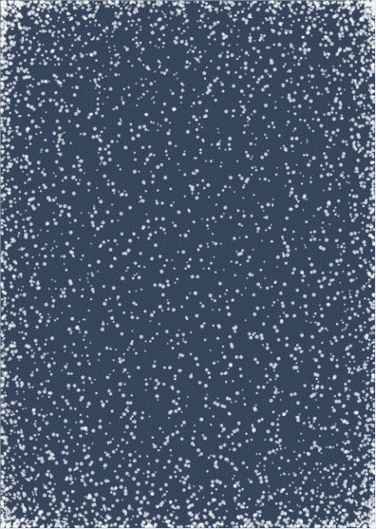
\includegraphics[width=3.3cm]{../pic/diffusion_static.png}
            \caption{Microscopic view}
        \end{figure}
        \column{0.5\textwidth}
        - Random Brownian Motion as they diffuse \\
        - Follows a small Gaussian distribution \\
        - reverse process also follows a Gaussian distribution
    \end{columns}
\end{frame}


\section{Theory}
\begin{frame}{The Process of DDPM}
    \begin{figure}[htbp]
        \centering
        \subfloat[Initial]
        {
            \begin{minipage}[b]{.3\linewidth}
                \centering
                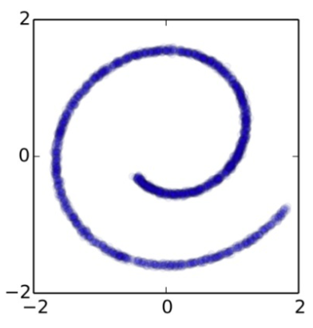
\includegraphics[scale=0.5]{../pic/1.png}
            \end{minipage}
        }
        \subfloat[Add noise]
        {
            \begin{minipage}[b]{.3\linewidth}
                \centering
                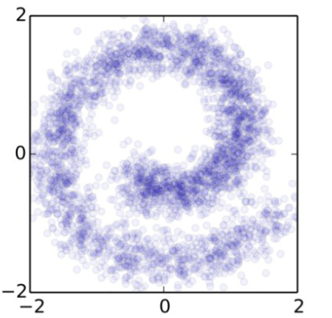
\includegraphics[scale=0.5]{../pic/2.png}
            \end{minipage}
        }
        \subfloat[Final]
        {
            \begin{minipage}[b]{.3\linewidth}
                \centering
                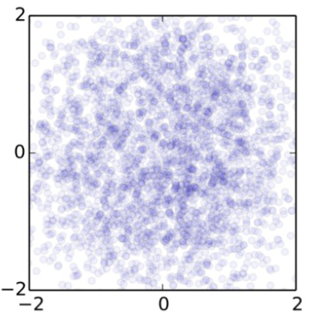
\includegraphics[scale=0.5]{../pic/3.png}
            \end{minipage}
        }
        \caption{how the figure tranform to a Gaussian Distribution}
    \end{figure}
\end{frame}

\begin{frame}{Forward Equation}
    \begin{block}{Forward}
        \begin{equation}
            q(x_t|x_{t-1}) = N(x_t;x_{t-1}\sqrt{1-\beta t}, I\beta_t)
        \end{equation}
        \begin{equation}
            x_t = x_{t-1} \sqrt{1-\beta_t} +  z_t\sqrt{\beta_t}
        \end{equation}
    \end{block}
    \begin{block}{}
        \begin{align*}
            x_t & = x_{t-1} \sqrt{1-\beta_t}+ z_t\sqrt{\beta_t} \ \ \ ({\rm let\ } 1-\beta_t = \alpha_t) \tag{1a}                              \\
                & = x_{t-2} \sqrt{\alpha_t}(\sqrt{\alpha_{t-1}} + z_{t-2} \sqrt{1-\alpha_{t-1}}) + z_{t-1}\sqrt{1-\alpha_t}   \tag{2a}         \\
                & = x_{t-2} \sqrt{\alpha_t\alpha_{t-1}}  + z_{t-2} \sqrt{\alpha_t - \alpha_t\alpha_{t-1}} + z_{t-1} \sqrt{1-\alpha_t} \tag{3a} \\
                & = x_{t-2} \sqrt{\alpha_t\alpha_{t-1}} + z\sqrt{1-\alpha_t\alpha_{t-1}}                                          \tag{4a}     \\
                & = \cdots                                                                                                                     \\
                & = x_0 \sqrt{\bar{\alpha_t}} + z\sqrt{1-\bar{\alpha_t}}\tag{5a}
        \end{align*}
    \end{block}
\end{frame}

\begin{frame}
    \frametitle{Backward Equation}
    \begin{block}{}
        \begin{align*}
            q(x_{t-1} | x_t, x_0) & = q(x_t | x_{t-1}, x_0) \frac{q(x_{t-1}|x_0)}{q(x_t|x_0)} \\
                                  & \propto \exp\left(
            - \frac 12 \left(
            \textcolor{red} { (\frac{\alpha_t}{\beta_t}
                + \frac 1{1-\bar{\alpha}_{t-1}}) } x_{t-1}^2
            \textcolor{blue}{ - (\frac{2\sqrt{\alpha_t}}{\beta_t}x_t
                + \frac{2\sqrt{\bar{\alpha}_{t-1}}} {1-\bar{\alpha}_{t-1}} )} x_{t-1}
            +C(x_t, x_0) \right)
            \right)                                                                           \\
                                  & = \exp \left ( -\frac12
            \left ( \textcolor{red}{A} x_{t-1}^2 + \textcolor{blue}{B} x_{t-1} + C \right )
            \right )
        \end{align*}
        \begin{equation}
            \mu = -\frac{\textcolor{blue}{B}}{2\textcolor{red}{A}}, \sigma^2 = \frac {1}{\textcolor{red}{A}}
        \end{equation}
    \end{block}
    \begin{block}{Backward}
        \begin{equation}
            p(x_t|x_{t-1}) = N(x_{t-1};f_\mu(x_t, t),f_\sigma^2(x_t, t))
        \end{equation}
    \end{block}
\end{frame}

\section{Features}

\begin{frame}{DDPM Features}
    \begin{table}
        \begin{tabular}{| c || c | c | c | c | c |  }
            \hline
            Name.      & Likelihood & Speed & Methods    & Stability & Others       \\
            \hline \hline
            GANs       & None       & fast  & One-step   & Unstable  & high quality \\
            VAEs       & Uncertain  & fast  & One-step   & Stable    & -            \\
            Flow Model & Exactly    & fast  & Multi-step & Stable    & -            \\
            DDPM       & Uncertain  & slow  & Multi-step & Stable    & beat GANs    \\
            \hline
        \end{tabular}
        \caption{Comparision of generative model}
    \end{table}
\end{frame}

\begin{frame}{Beat GANs}
    \centering
    \begin{figure}
        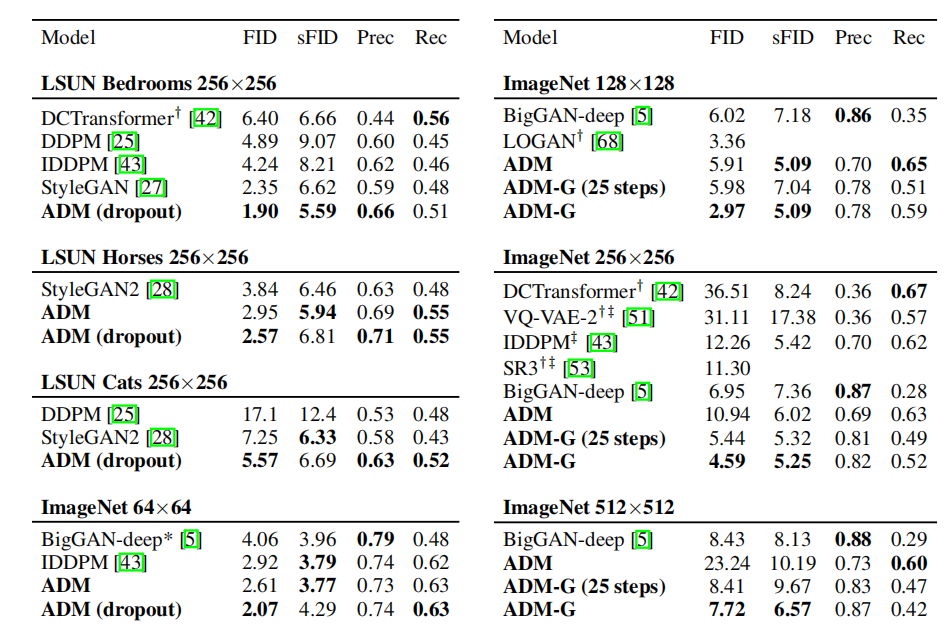
\includegraphics[height=4.5cm]{../pic/beat-GANs.png}
        \caption{Some data about beat GANs}
    \end{figure}
\end{frame}



\section{Application}

\begin{frame}{Text2Image}
    Generate images that match the description from the text, give some descriptions, and generate pictures that meet the description.
    \begin{figure}
        \centering
        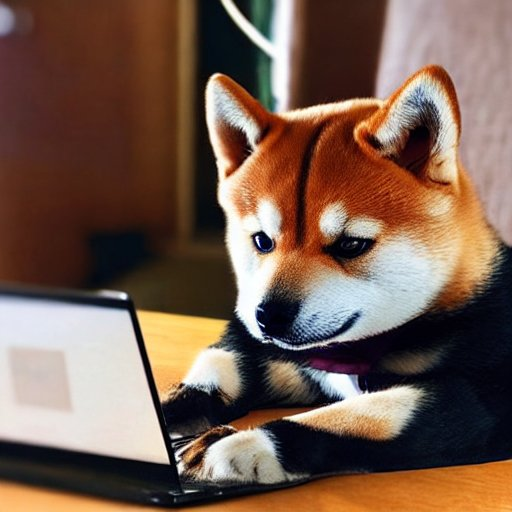
\includegraphics[height=4.5cm]{../pic/dog-is-reading.png}
        \caption{A dog is reading book}
    \end{figure}
\end{frame}

\begin{frame}{Image Refinement}
    Refine the blurry image to give the picture more detail.
    \begin{figure}
        \centering
        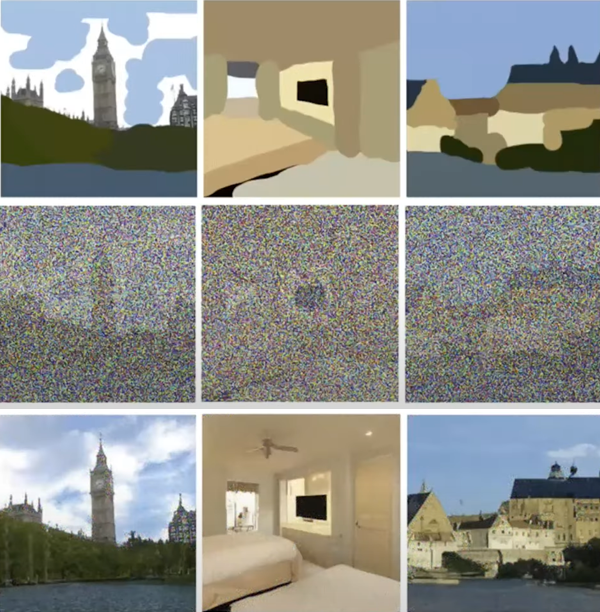
\includegraphics[height=4.5cm]{../pic/compose.png}
        \caption{Image Refinement with Diffusion}
    \end{figure}
\end{frame}
\begin{frame}{Inpainting}
    Padding the missing image can complement the details and content of the image.
    \begin{figure}
        \centering
        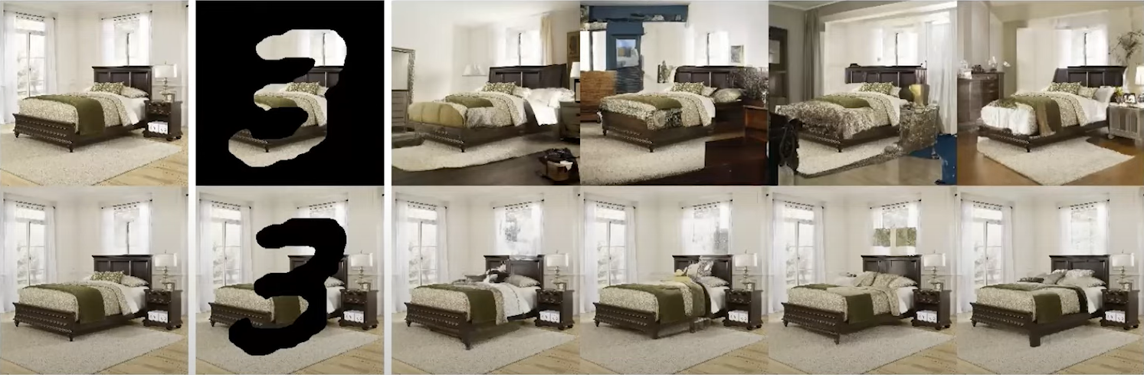
\includegraphics[height=4.5cm]{../pic/inpainting.png}
        \caption{inpainting with Diffusion}
    \end{figure}
\end{frame}
\begin{frame}{Colorization}
    Color fill images with missing colors.
    \begin{figure}
        \centering
        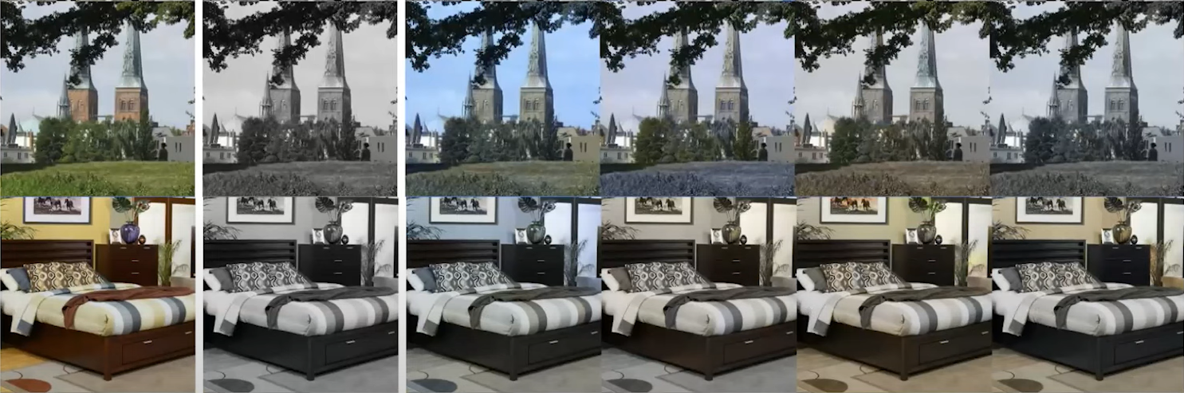
\includegraphics[height=4.5cm]{../pic/colorization.png}
        \caption{Colorization with Diffusion}
    \end{figure}
\end{frame}
\section{Conclusion}

\begin{frame}{Worries and Prospect}
    \begin{block}{Worries}
        malicious uses for political purposes
    \end{block}
    \begin{block}{Prospect}
        uses in art, photography, and music
    \end{block}
\end{frame}
\section*{References}
\begin{frame}{References}
    Thank you for watching!
    \vfill
    Here is the \textbf{References}
    \begin{itemize}
        \item Ho J, Jain A, Abbeel P. Denoising diffusion probabilistic models[J]. Advances in Neural Information Processing Systems, 2020, 33: 6840-6851.
        \item Dhariwal P, Nichol A. Diffusion models beat gans on image synthesis[J]. Advances in Neural Information Processing Systems, 2021, 34: 8780-8794.
    \end{itemize}
    \vfill
    \rightline{Edit with \LaTeX}
\end{frame}

\end{document}